\section{Results}



\paragraph{\gear achieves state-of-the-art performance in multi-step retrieval}
The multi-step section of Table \ref{tab:recall_main_table} demonstrates that our agent setup for enabling multi-step retrieval is highly effective, achieving state-of-the-art performance across all datasets. While we observe significant improvements on saturated datasets like 2Wiki and HotpotQA, \gear particularly excels on the MuSiQue dataset, delivering performance gains exceeding 10\% over the competition.


\begin{figure}[t]
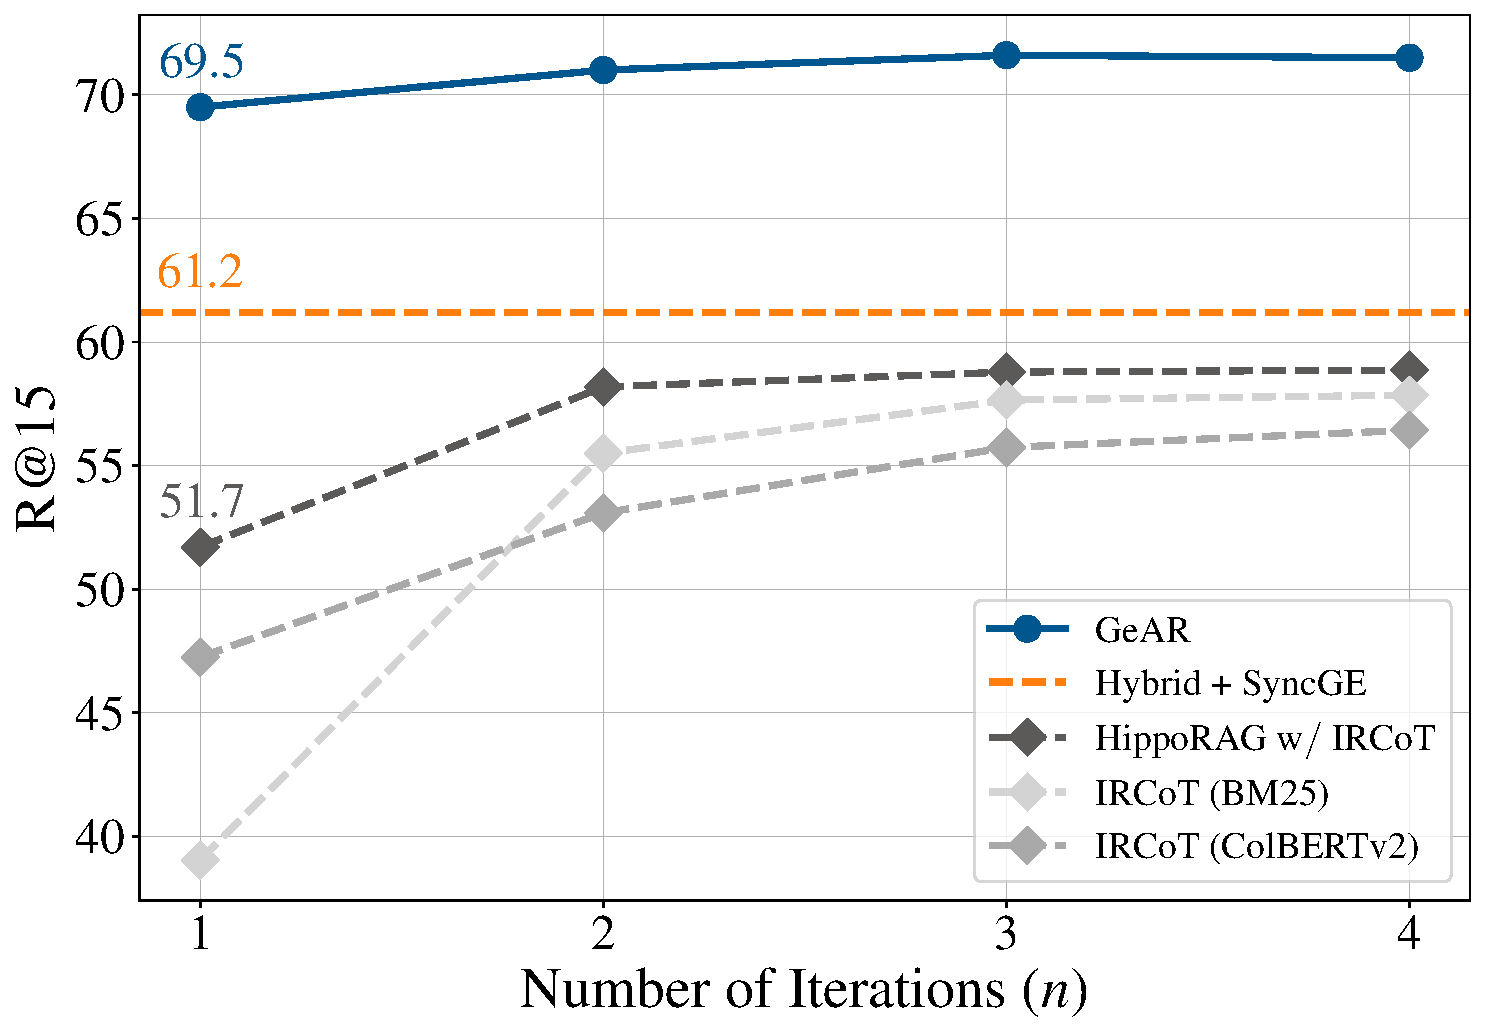
\includegraphics[width=\columnwidth]{figures/experiments/recall_evolution_across_agent_iterations_4_iters.pdf}
\caption{\label{fig:recall_across_iterations}R@15 evolution over $4$ iterations on MuSiQue. Recall is computed at each iteration using the cumulative set of retrieved documents, with prior recall values carried forward for questions that terminated in earlier iterations. The horizontal line indicates the single-step performance of Hybrid + SyncGE.}
\end{figure}

\paragraph{SyncGE contributes to state-of-the-art performance in single-step retrieval}
As shown in the single-step section of Table \ref{tab:recall_main_table}, our proposed Hybrid + SyncGE method achieves state-of-the-art single-step retrieval performance on both MuSiQue and HotpotQA datasets. We observe consistent improvements using NaiveGE and SyncGE, outperforming HippoRAG in many setups regardless of the base retriever (i.e. sparse, dense or hybrid). Most notably, Hybrid + SyncGE surpasses HippoRAG by up to $9.8\%$ at R@15 on MuSiQue.




\paragraph{Higher recall leads to higher QA performance}Aligning with findings from prior works, our analysis reveals a consistent correlation between recall and QA performance \cite{Gutierrez2024}. As shown in Table \ref{tab:em_and_f1}, \gear achieves the highest EM and F1 scores. A closer examination of relative improvements yields interesting insights. Taking MuSiQue as an example, \gear shows a $21\%$ relative improvement in R@15 compared to HippoRAG w$/$ IRCoT, while achieving a $37\%$ relative improvement in both EM and F1 scores. Mirroring the pattern observed in Table~\ref{tab:recall_main_table}, its graph-based retriever (i.e. SyncGE) outperforms HippoRAG on both MuSiQue and HotpotQA.

\begin{table}[thbp]
\small
\setlength{\tabcolsep}{3pt}
  \centering
  \small
\begin{tabular}{L{2.3cm}cccccc}
\toprule \multirow{2.5}{*}{\textbf{Retriever}} & \multicolumn{2}{c}{\textbf{MuSiQue}} & \multicolumn{2}{c}{\textbf{2Wiki}} & \multicolumn{2}{c}{\textbf{HotpotQA}} \\ \cmidrule{2-7} & EM  & F1 & EM & F1 & EM & F1 \\ \midrule
\rowcolor[gray]{0.9} No Passages & $2.6$ & $12.5$& $17.2$ & $27.9$ & $19.5$ & $34.3$ \\
\rowcolor[gray]{0.9} Gold Passages & $36.6$ & $59.2$ & $54.4$ & $70.3$ & $55.0$ & $75.9$  \\ \midrule
Hybrid + SyncGE & $14.0$ & $\underline{27.1}$ & $38.0$ & $50.2$ & $45.0$ & $63.4$ \\
HippoRAG & $8.2$ & $18.2$ & $39.8$ & $51.8$ & $40.1$ & $57.6$ \\ \midrule
IRCoT (BM25)& $7.6$ & $15.9$ & $28.8$ & $38.5$ & $34.3$ & $50.8$ \\ 
IRCoT (ColBERTv2) & $12.2$ & $24.1$ & $32.4$ & $43.6$ & $45.2$ & $63.7$ \\
HippoRAG w$/$ IRCoT & $\underline{14.2}$ & $25.9$ & $\underline{45.6}$ & $\underline{59.0}$ & $\underline{49.2}$ & $\underline{67.9}$ \\ 
\gear & $\mathbf{19.0}$ & $\mathbf{35.6}$ & $\mathbf{47.4}$ & $\mathbf{62.3}$ & $\mathbf{50.4}$ & $\mathbf{69.4}$ \\ \bottomrule
\end{tabular}
\caption{End-to-end QA performance using the  top-$5$ retrieved passages. The \textbf{best} model is in bold and \underline{second best} is underlined. The top part shows the lower and upper bounds of QA performance, while the middle and bottom sections display scores for single-step and multi-step retrievers, respectively.}
\label{tab:em_and_f1}
\end{table}
